\section{Introduction}
% Making Abstraction Concrete
We communicate with others at all stages of creative work, from ideation to critique \cite{mamykina2002collaborative}. 
For example, when writing, collaborators often first generate a high-level outline, later shifting focus to a lower level by revising grammar \cite{sommers1980revision}. Visual work like web design also spans abstraction levels, from task goals to deciding specific element placement \cite{klemmer2001designers}. Early on, high-level concerns should dominate. For example, in drawing, exploring various compositions early is more important than deciding what specific characters look like. Lightweight sketches serve as exploratory tools to visually communicate ideas in domains from architecture to illustration \cite{Buxton2007,Tversky2011,Tversky2009}. Dancers use marking to physically think through choreography without focusing on the details of the dance \cite{kirsh2011marking}. Designers use paper prototyping \cite{Snyder2003} and storyboarding \cite{landay1996sketching} to collaboratively think through a goal without focusing heavily on concrete details. These `blocking' strategies help people view work as high-level chunks rather than individual elements \cite{Chase1973,Gobet1998,chi1981categorization} While abstract chunking and high-level exploration are important for both ideation and collaboration, the emphasis of online collaboration in creative tasks has been on refinement and revision of completed work. Focusing on details early on can shift a group's attention to refinement rather than rough exploration, which can lead to fixation on a single idea \cite{jansson1991design,simon1972theories} or iterating incrementally on a previous idea rather than trying a potentially new and better concept \cite{Dow2009,Little2010,Yu2016}. 

We know that abstraction helps \emph{individuals} focus on high-level concerns \cite{Chase1973}; a combination of early stage abstraction and structure may also help \emph{collaborators} focus on high-level ideation and communicate with one another. We hypothesize that explicitly supporting `chunks' for early-stage design catalyzes collaborators' ability to revise at an appropriate level of abstraction by breaking down sketches into discrete, adaptable parts. Inspired by expert uses of chunking and tools that use tangible interfaces and techniques \cite{klemmer2001designers,Resnick2009}, this chapter investigates using abstract blocks as a form of visual chunking and a tool for structuring group communication. 
For example, a drawing of a tourist at a train station might consist of several abstract blocks to represent placement of these elements (Figure \ref{fig:blocks}); these blocks can be directly manipulated to communicate desired changes, suggestions, or ideas without the immediate need to change the sketch itself. Users can choose to label the blocks either through text or pictorially, giving flexibility in how they choose to represent their ideas. We focus on sketching as an initial exemplar domain of the broader class of creative work because sketching is an easily accessible medium that only requires pen and paper and is a beneficial tool for visual communication \cite{Buxton2007,Tversky1999}.

\begin{figure}
\centering
  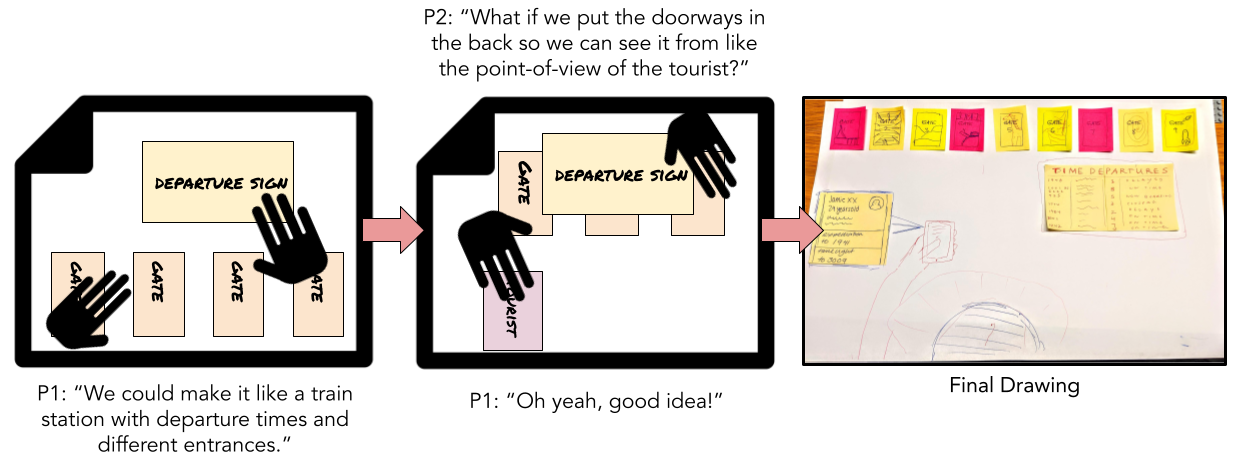
\includegraphics[width=\textwidth]{abstraction/figures/main_fig.png}
  \caption[A group from our study discussed composition and layout ideas for a collaborative sketch using abstract blocks.]{A group from our study discussed composition and layout ideas for a collaborative sketch using abstract blocks. These tangible and malleable blocks remove the need for smaller details and emphasize exploration. The prompt for the sketch was ``A scene with a time-travelling tourist.''}~\label{fig:blocks}
\end{figure}

% We hypothesize that this form of structured abstraction helps groups break down sketches into discrete, adaptable parts to communicate high-level ideas.
%---
%THINKING WiTH BOXES

An observational study investigated abstract blocks in a collaborative task. Six groups of novices ($n=19$) created drawings collaboratively. We audio and video recorded sessions and interviewed groups in a retrospective think-aloud. Groups used a paper implementation of abstraction blocks, using sticky notes, to plan a sketch based on a prompt. Working with simple blocks helped groups to see their drawings in terms of malleable, conceptual chunks. Tangible blocks helped groups discuss high-level concepts like `point-of-view` or `scale` and helped them quickly explore and change the composition of the drawing by editing the configuration of the blocks. Working at this more abstract, block level appeared to keep early discussion on more conceptual discussion rather than lower-level implementation details. These results suggest to us that offering (or even enforcing) abstract creation primitives like blocks catalyzes an emphasis on strategic and conceptual issues. 

